%!TEX root = FreeRtos ARM uController.tex
\subsection{Intertask Kommunikation}
%Michael: Ich habe in diesen Abschnitten nichts verändert, nur ein paar Kommentare. Vielleicht sollten wir noch etwas an Beispielen einbringen, wie von Frau Ma empfohlen hat. Zur Zeit ist es ne ziemliche wall of text :) 
In Projekten, in denen verschiedene Tasks parallel verarbeitet werden, ist es häufig erforderlich, dass diese Tasks die Möglichkeit besitzen Informationen untereinander auszutauschen. Zum Einen kann ein Task Informationen produzieren, die ein anderer Task für die weitere Verarbeitung benötigt. Zum Anderen können beide Tasks gemeinsame Ressourcen (z.B. Hardwareregister oder Variablen) nutzen. Hierbei muss sichergestellt werden, dass die dort hinterlegten Daten jederzeit korrekt sind. FreeRTOS bietet hierfür verschiedene Funktionen zur Interprozesskommunikation an.\newline Zuerst sind hier die Queues zu nennen. Diese dienen dem klassischen Austausch von Informationen, indem Daten durch einen Task in die Queue hineingeschrieben werden und von einem zweiten Task gelesen werden. Die Größe der Queue wird beim Aufruf der Erzeugerfunktion definiert. In FreeRTOS wird eine Queue mit folgender Funktion erstellt: 
\begin{lstlisting}[numbers = none]
xQueueCreate(uxQueueLength,uxItemSize)
\end{lstlisting}
Es werden keine expliziten Queues angeboten, die Pointer speichern. Es ist jedoch möglich Pointer als Datum in einer Queue zu hinterlegen. Um einen Überlauf der Queue zu verhindern, werden Tasks, die in eine volle Queue hineinschreiben wollen, in den Zustand Blocked versetzt. Ebenso werden Tasks behandelt, die versuchen Daten aus einer leeren Queue abzurufen. Um die Echtzeitfähigkeit der Tasks weiter zu gewährleisten, bieten die Funktionen xQueueSendToFront(), xQueueSendToBack() und xQueueReceive() einen Parameter xTicksToWait an. Mit xTicksToWait übergibt ein Task den Zeitwert, in dem der Task eine Antwort erwartet. Erfolgt innerhalb dieser Zeit keine Antwort, so wird der Task mittels Rückgabewert über diesen Timeout informiert.
Wenn mehrere Tasks auf eine gemeinsame Queue zugreifen, wird deren Zugriff im o.g. Fall zuerst nach Priorisierung des Tasks und danach durch Wartezeit gesteuert. Je nach Zustand der Queue erhält der Task mit der höchsten Priorität den Zugriff. Existieren zwei Tasks mit der gleichen Priorität, so darf der Task zugreifen, der schon länger auf einen Zugriff wartet\cite[p.101ff]{MasteringFreeRtos}.\newline
Queues bieten außerdem die Möglichkeit als Mailbox konfiguriert zu werden. In diesem Fall verhalten sich grund\-sätz\-lich wie Queues, beinhalten jedoch nur ein Datenobjekt. Dieses wird nach dem Lesen nicht direkt gelöscht, sondern verbleibt in der Mailbox, bis es von einem datenerzeugenden Task über\-schrie\-ben wird. Mailboxen sind vor allem in Szenarien interessant, in denen mehrere Tasks lesend auf ein erzeugtes Datum zugreifen sollen. Beispielsweise greift ein Task zur Verarbeitung und ein niedriger priorisierter Task zur Anzeige auf die Mailbox zu\cite[p.143ff]{MasteringFreeRtos}.
\newline
FreeRTOS bietet außerdem Semaphore an. Semaphore werden im Rahmen der Interprozesskommunikation meist zur Synchronisierung der Tasks (mit einem anderen Task oder einem Interrupt) angewendet. 
Hierzu wird durch einen Task der Semaphor angefordert und durch den zweiten Task der Semaphor gesetzt. Semaphore werden detailliert im Abschnitt \ref{sec:Interrupt} beschrieben.
\newline
Die nächste Gruppe der Funktionen zur Interprozesskommunikation sind die Mutexe. Diese bilden eine Sonderform der Semaphore und sind nahezu identisch implementiert. 
Mutexe werden benutzt um Zugriffe auf gemeinsam genutzte Ressourcen zu steuern. Wenn ein Task auf eine Ressource zugreifen will, so prüft er vorher, ob er den Mutex erhalten kann. Ist dies nicht der Fall, weil ein anderer Task den Mutex besitzt, so muss der Task warten bis der andere Task den Mutex zurück gibt. 
Im Gegensatz zu Semaphoren bieten Mutexe die Möglichkeit einen Task, der den Mutex besitzt kurzzeitig höher zu priorisieren, sodass eine zeitnahe Abarbeitung stattfinden kann. Hierdurch können Wartezeiten von hoch priorisierten Tasks auf niedriger priorisierte Tasks reduziert werden. Es kann jedoch zu Laufzeitproblemen kommen.  
\begin{figure}[ht!]
	\centering
		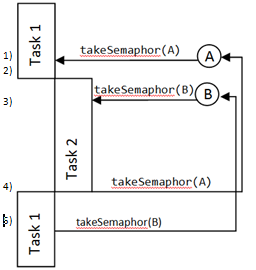
\includegraphics[width=0.2\textwidth]{Pictures/Intertask/Deadlock.png}
	\caption{Entstehung eines Deadlocks. 1) Task 1 erhält Mutex A; 2) Task 1 wird im Rahmen des Schedulings verdrängt, Task 2 wird aktiv; 3) Task 2 erhält Mutex B; 4) Task 2 versucht Mutex A zu erhalten, dieser ist durch Task 1 belegt. Task 2 wird daher in den Zustand "`Wait"' versetzt und Task 1 wird wieder gestartet 5) Task 1 versucht Mutex B zu erhalten, dieser ist durch Task 2 belegt. Der Deadlock entsteht.}
	\label{fig:Deadlock}
\end{figure}

Bei der Verwendung von Mutexen können Deadlocks entstehen (Abbildung \ref{fig:Deadlock}). Hierbei versuchen zwei, oder mehr Tasks zeitgleich auf zwei, oder mehr Ressourcen zuzugreifen. Beiden Tasks gelingt es mindestens einen Mutex zu erhalten. In Folge kann keiner der Tasks vollen Zugriff auf die Ressourcen erlangen und wartet jeweils auf den anderen. Der Deadlock kann nur aufgebrochen werden, indem einer der Tasks seine Mutexe zurück gibt und der andere diese erhalten kann\cite[p.243ff]{MasteringFreeRtos}. 
Durch die notwendigen Timeouts kann die Echt\-zeit\-fähig\-keit des Systems sichergestellt werden. 
Die Entwickler von FreeRTOS verwenden daher Wrapper-Funktionen, auch Gatekeeper genannt (Abbildung \ref{fig:Gatekeeper}). Diese nehmen eine Kapselung der Ressourcen vor und werden über Queues angesprochen. Auf diesem Weg kann auf den Einsatz von Mutexen weitestgehend verzichtet werden\cite[p.259ff]{MasteringFreeRtos}.
\begin{figure}[ht!]
	\centering
		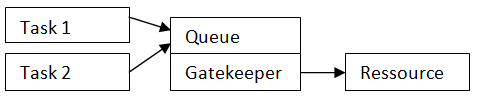
\includegraphics[width=0.3\textwidth]{Pictures/Intertask/Gatekeeper.png}
	\caption{Zugriff von verschiedenen Tasks auf eine Ressource mittels einer Gatekeeper-Task.}
	\label{fig:Gatekeeper}
\end{figure}
Die dritte Form der Intertaskkommunikation, die von FreeRTOS angeboten wird, ist die Task Notification. Sie ist die Variante mit dem geringsten Ressourcenaufwand, da anders als bei Queues und Mutexes keine Datenobjekte angelegt werden müssen. Durch das Aktivieren der Task Notifikation innerhalb der FreeRTOSConfig.h durch das Setzen von 
\begin{lstlisting}[numbers = none]
#define configUSE_TASK_NOTIFICATIONS 1
\end{lstlisting}
wird pro Task ein fester Speicherbereich reserviert, der für die Notification genutzt wird. Task Notifications werden direkt an den Zieltask gesendet. Es findet, anders als bei Queues, kein Zwischenspeichern der Information statt. Wenn ein Task einen anderen Task benachrichtigt, wird diese in den Zustand Blockiert versetzt, bis der Notification Wert in den hierfür vorgesehen Speicherbereich geschrieben wurde. Darüber hinaus ist bei Notifications sichergestellt, dass die Informationen ausschließlich zwischen den beiden beteiligten Tasks ausgetauscht werden. Ein Zugriff eines dritten Tasks oder einer Interrupt Service Routine (ISR) auf diese Kommunikation ist ausgeschlossen\cite[p.293ff]{MasteringFreeRtos}.
